\documentclass[12pt]{article}
   
\usepackage[utf8]{inputenc}
   \usepackage{graphicx}
   \usepackage{float}
   \usepackage{subcaption}
   %\usepackage{mathtools}
   \usepackage{amsmath}
   
   \addtolength{\hoffset}{-0.7in}
   \addtolength{\textheight}{1.5in}
   \addtolength{\textwidth}{1.5in}
   \addtolength{\voffset}{-1in}
%
% Title.
\title{EE230: Experiment 4\\
Instrumentation Amplifier on load cell sensor}

% Author
\author{Hitesh Kandala, 180070023}

% begin the document.
\begin{document}

% make a title page.
\maketitle

\section{Overview of the experiment}

    \subsection{Aim of the experiment}
        \begin{itemize}
            \item In this experiment, we wish to implement instrumentation amplifier to amplify output from a load cell sensor. This is done in two parts:
            \begin{itemize}
                \item In part 1, we build the instrumentation amplifier using TL084 IC.
                \item In part 2, we implement the instrumentation amplifier using INA128 IC.
            \end{itemize}
            \item To observe/compare the output from the above two methods.
        \end{itemize}

    \subsection{Theory}
        \subsubsection{Load Cell}
            A load cell is based on an electrical circuit called Wheatstone bridge. It consists of 4 strain gauges connected on a cantilever beam that undergo change in resistance when deformed (i.e. when the object they are connected to experiences strain).
            \begin{figure}[H]
                \centering
                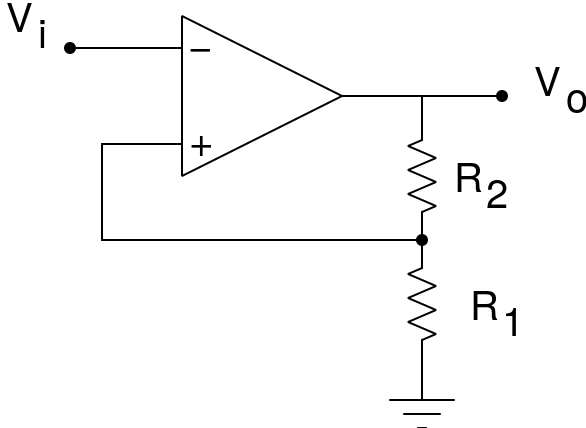
\includegraphics[width = 0.4\linewidth, height = 1.8in]{reports/lab2/non.png}
                \caption{Schmitt trigger}
            \end{figure}
            \\
            \noindent
            This arrangement allows to measure very small changes in the resistance R, which occurs in the strain gauges placed in the arms of the bridge: R1, R2, R3 and R4. When the load cell has no load, the four gauges are at rest and have the same ohmic value, the nominal value of the strain gauge Rg:
            \begin{equation}
                R_1 = R_2 = R_3 = R_4 = R_g 
            \end{equation}

            \begin{figure}[H]
                \centering
                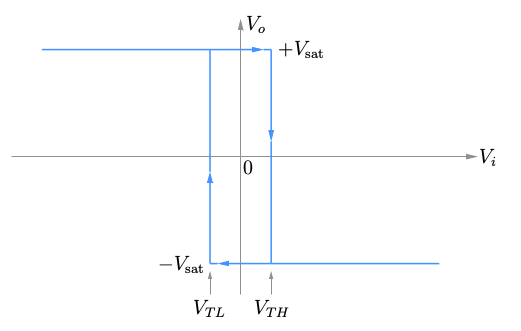
\includegraphics[width = 0.7\linewidth, height = 3in]{reports/lab2/scmiii.png}
                \caption{$V_o$ versus $V_i$ relationship for Schmitt trigger}
            \end{figure}
            \noindent
            When the load cell experiences deformation due to externally applied force, the resistance of each strain gauge changes by a very small amount ∆R: (when the force is not large enough to make the response of the sensors non-linear).
            \begin{equation}
                R_1 = R_g + \Delta R; R_2 = R_g - \Delta R; R_3 = R_g - \Delta R; R_4 = R_g + \Delta R; 
            \end{equation}
    
        \subsubsection{Instrumentation Amplifier}
            An instrumentation amplifier is a type of differential amplifier that has been outfitted with input buffer amplifiers. These input buffers eliminate the need for input impedance matching and thus make the amplifier particularly suitable for use in measurement and test equipment. Additional characteristics include very low DC offset, low drift, low noise, very high open-loop gain, very high common-mode rejection ratio, and very high input impedance. Instrumentation amplifiers are used to achieve high accuracy and stability.
            \\
            
            \noindent
            Here, we define the input voltage signals small signal AC differential input $V_1$ and $V_2$, as the input of first stage OPAMPs of the instrumentation amplifier. We assume input resistance of OPAMPs to be infinite. Now applying KCL at inverting input of first stage OPAMPs. We get,
            \begin{equation}
                V_a = V_1(1 + R_2/R_1) + V_2(R_2/R_1)
            \end{equation}
            \begin{equation}
                V_b = - V_1(R_2/R_1) + V_2(1 + R_2/R_1)
            \end{equation}
            Using superposition principle of voltages at second stage OPAMP,
            \begin{equation}
                V_{out} = R_4/R_3(1 + 2R_2/R_1)(V_2 - V_1)
            \end{equation}
            The gain is
            \begin{equation}
                A_v = \frac{V_{out}}{V_1 - V_2} = \frac{R_4}{R_3}(1 + \frac{2R_2}{R_1})
            \end{equation}
            
    
\newpage
\section{Experimental results}

    \subsection{Part 1 : Using Operational amplifier TL084}
        \begin{figure}[H]
            \centering
            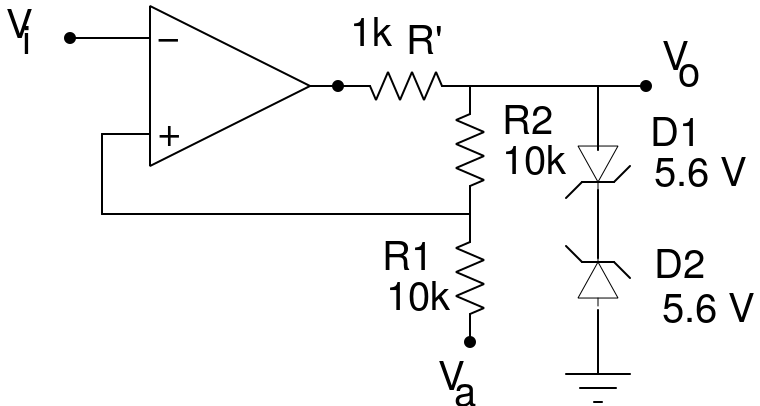
\includegraphics[width = 0.7\linewidth, height = 2.6in]{reports/lab2/scmidt.png}
            \caption{Schmitt trigger}
        \end{figure}
        
        % \begin{figure}[H]
        %     \centering
        %     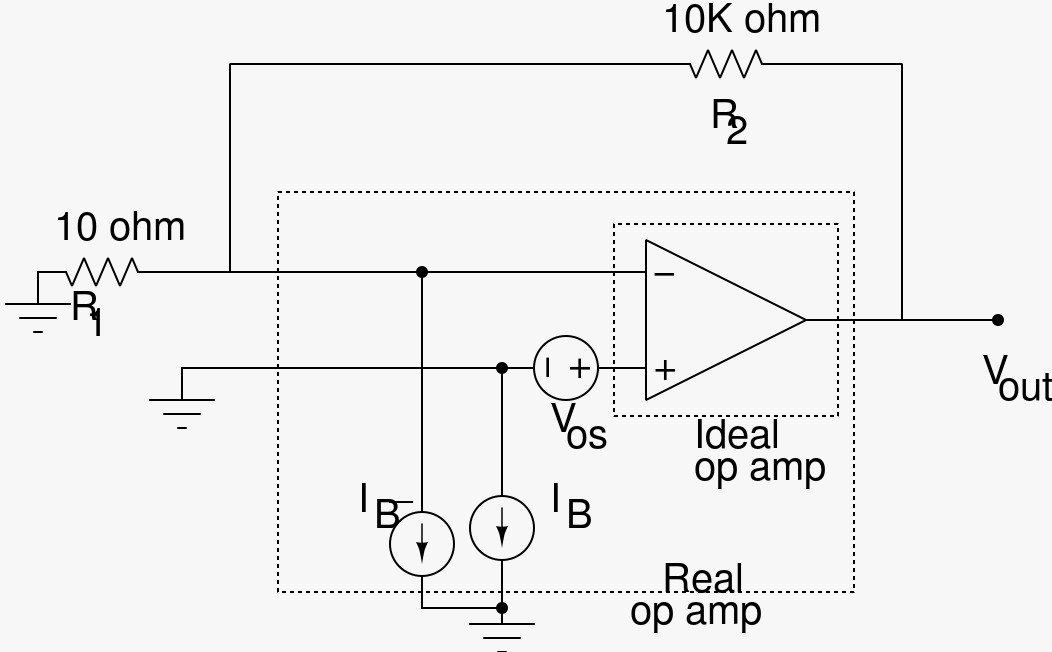
\includegraphics[width = 0.8\linewidth, height = 2.5in]{offset_real.jpeg}
        %     \caption{Equivalent circuit}
        % \end{figure}
        
    %   \textbf{(A) With $\mathbf{V_{a} = 0V :}$}\\
         
    %     \begin{equation}
    %         V_{TL} = -V_{sat} \times (\frac{R_1}{R_1 + R_2}) 
    %     \end{equation}
    %     \\
    %     \begin{equation}
    %         V_{TH} = +V_{sat} \times (\frac{R_1}{R_1 + R_2}) 
    %     \end{equation}
    %     \\
    %     The actual resistance of resistors shown in fig 5 are,
    %     $R_1 = 9.7k$, $R_2 = 9.82k$, $R' = 0.96k$
    %     \\
    %     Drop across zener diodes is $V_{Z} + V_{ON} = 5.6V + 1.12V = 6.72V$\\
        % \begin{equation}
        %     V_{TL} = -6.72 \times (\frac{9.7}{9.7 + 9.82})
        % \end{equation}
        % \begin{equation}
        %     \boxed{V_{TL} = -3.34V}
        % \end{equation}
        % Similarly,
        % \begin{equation}
        %     \boxed{V_{TH} = +3.34V}
        % \end{equation}
        
        Hence, theoretical values of $\mathbf{V_{TH}}$ and $\mathbf{V_{TL}}$ are \textbf{+3.34V} and \textbf{-3.34V}   respectively.
        \\
        
        \begin{figure}[H]
            \centering
            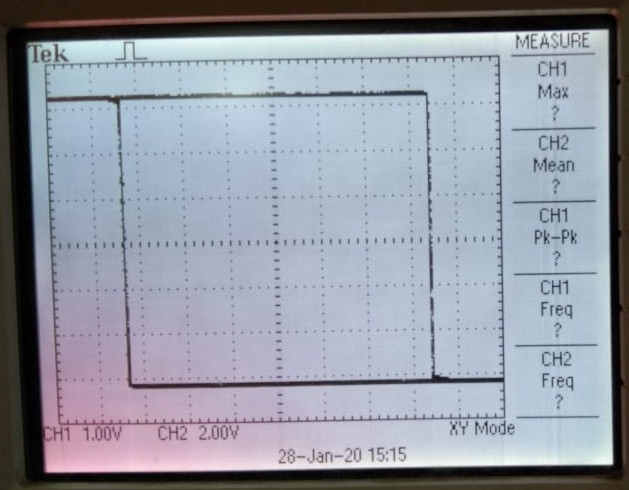
\includegraphics[width = 0.8\linewidth, height = 3in]{reports/lab2/scmidtt.jpeg}
            \caption{$V_o$ versus $V_i$ relationship for $V_a = 0V$}
        \end{figure}
        \\
        The observed value of $\mathbf{V_{TH} = +3.4V}$ and $\mathbf{V_{TL} = -3.4V}$\\
        \\
        \textbf{(B) With $\mathbf{V_{a} = 3V :}$}\\
         
        \begin{equation}
            V_{TL} = -V_{sat} \times (\frac{R_1}{R_1 + R_2}) 
        \end{equation}
        \\
        \begin{equation}
            V_{TH} = +V_{sat} \times (\frac{R_1}{R_1 + R_2}) 
        \end{equation}
        \\
        The actual resistance of resistors shown in fig 5 are,
        $R_1 = 9.7k$, $R_2 = 9.82k$, $R' = 0.96k$
        \\
        Drop across zener diodes is $V_{Z} + V_{ON} = 5.6V + 1.12V = 6.72V$\\
        \begin{equation}
            V_{TL} = -6.72 \times (\frac{9.7}{9.7 + 9.82}) + 3 \times (\frac{9.82}{9.7 + 9.82})
        \end{equation}
        \begin{equation}
            \boxed{V_{TL} = -1.83V}
        \end{equation}
        Similarly,
        \begin{equation}
            V_{TH} = 6.72 \times (\frac{9.7}{9.7 + 9.82}) + 3 \times (\frac{9.82}{9.7 + 9.82})
        \end{equation}
        \begin{equation}
            \boxed{V_{TH} = +4.85V}
        \end{equation}
        \\
        Hence, theoretical values of $\mathbf{V_{TH}}$ and $\mathbf{V_{TL}}$ are \textbf{+4.85V} and \textbf{-1.83V}   respectively.
        \\
        
        \begin{figure}[H]
            \centering
            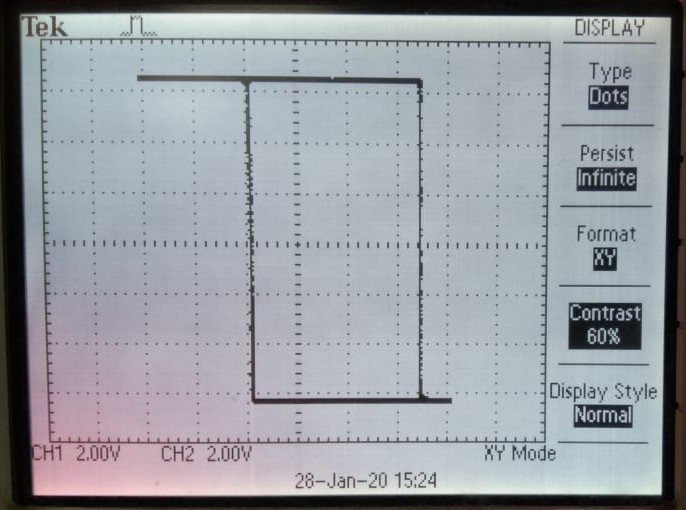
\includegraphics[width = 0.6\linewidth, height = 2.4in]{reports/lab2/scmidtt2.jpeg}
            \caption{$V_o$ versus $V_i$ relationship for $V_a = 0V$}
        \end{figure}
        \\
        The observed value of $\mathbf{V_{TH} = +4.8V}$ and $\mathbf{V_{TL} = -1.8V}$\\

\subsection{Astable multivibrator}
      \begin{figure}[H]
            \centering
            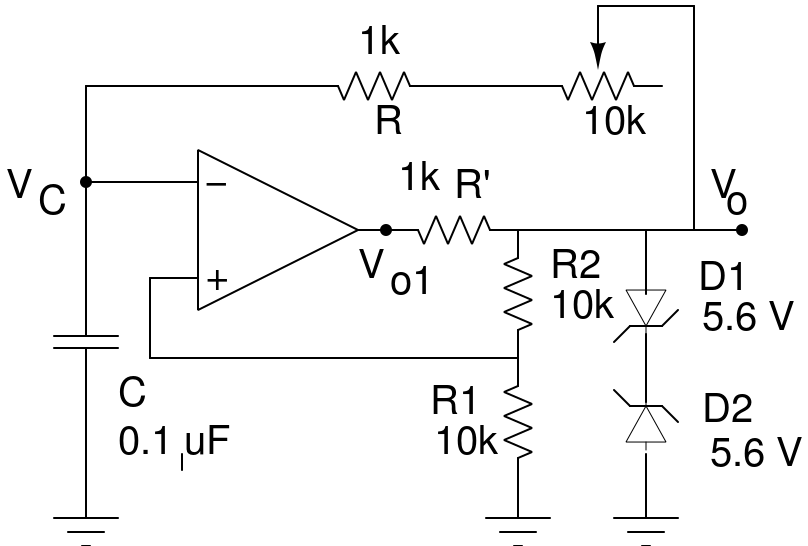
\includegraphics[width = 0.5\linewidth, height = 2.8in]{reports/lab2/astable.png}
            \caption{Astable multivibrator}
        \end{figure}
        \\
        The actual resistance of resistors shown in fig 8 are,
        $R_1 = 9.7k$, $R_2 = 9.82k$, $R' = 0.99k$, $R = 0.96k$\\
        \\
        \textbf{(A) For maximum time period :}\\
        \\
        The resistance between $V_C$ and $V_O$ comes out to be $\mathbf{10.73k \Omega}$
        \\
        Since here $V_a = 0V$,
        % \begin{figure}[H]
        %     \centering
        %     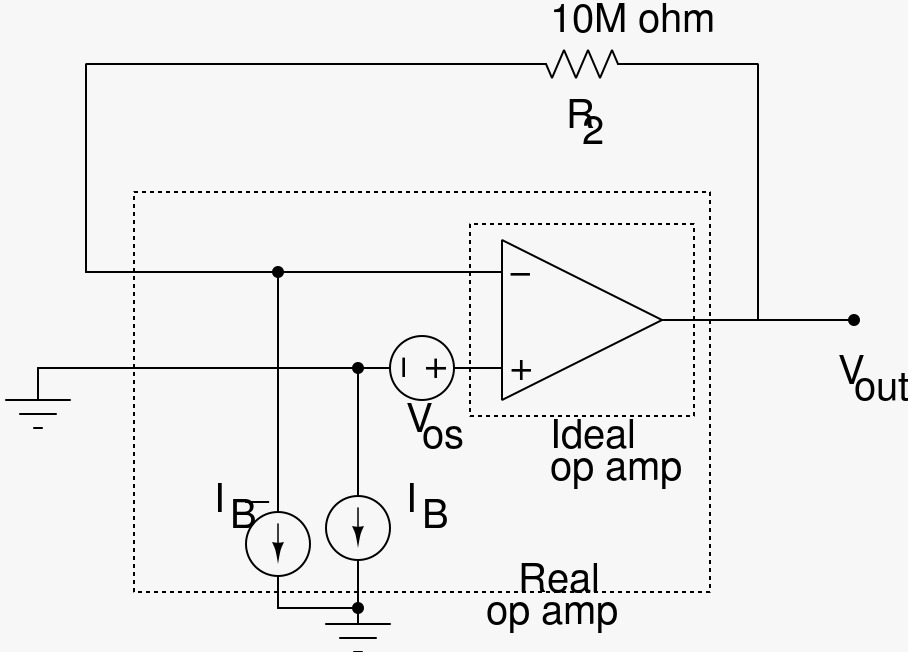
\includegraphics[width = 0.8\linewidth, height = 3in]{ibminusreal.jpeg}
        %     \caption{Equivalent internal circuit}
        % \end{figure}
        \begin{equation}
            V_{TH} = -V_{TL} \equiv V_{T}
        \end{equation}
        \\
        The period of oscillation is
        
        \begin{equation}
            T = 2\tau \log(\frac{V_m + V_T}{V_m - V_T}) \qquad \qquad where \quad \tau = RC
        \end{equation}
        \\
        \begin{equation}
            T = 2(10.73k)(0.1\mu) \log(\frac{6.72 + 3.4}{6.72 - 3.4})
        \end{equation}
        
        \begin{equation}
            \boxed{T = 2.39ms}
        \end{equation}
        \\
        \begin{figure}[H]
            \centering
            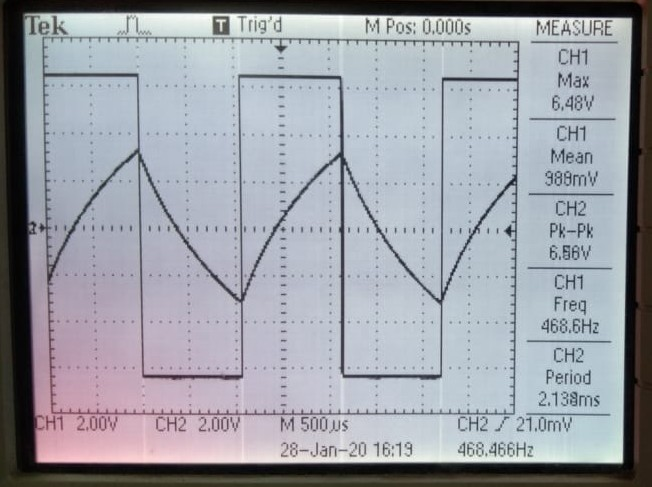
\includegraphics[width = 0.6\linewidth, height = 2.5in]{reports/lab2/astable.jpeg}
            \caption{Output for maximum time period}
        \end{figure}
        \\
        The observed maximum time period is $\mathbf{T = 2.138ms}$\\
        \\
        \textbf{(B) For minimum time period :}\\
        \\
        The resistance between $V_C$ and $V_O$ comes out to be $\mathbf{0.96k \Omega}$
        \\
        Again, the period of oscillation is given by
        
        \begin{equation}
            T = 2\tau\times \log(\frac{V_m + V_T}{V_m - V_T}) \qquad \qquad where \quad \tau = RC
        \end{equation}
        
        \begin{equation}
            T = 2\times(0.96k)\times(0.1\mu)\times \log(\frac{6.72 + 3.4}{6.72 - 3.4})
        \end{equation}
        
        \begin{equation}
            \boxed{T = 214\mu s}
        \end{equation}
        \\
        \begin{figure}[H]
            \centering
            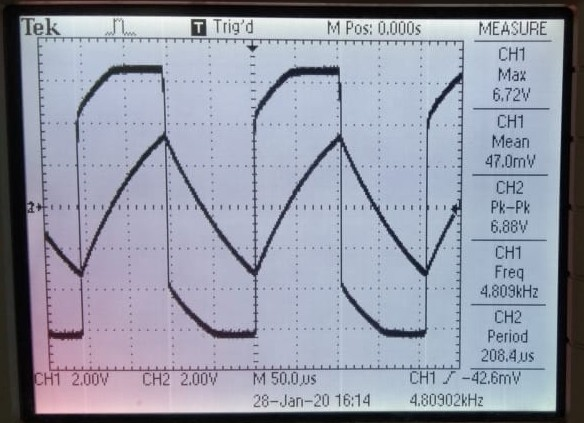
\includegraphics[width = 0.6\linewidth, height = 2.5in]{reports/lab2/astableMin.jpeg}
            \caption{Output for minimum time period}
        \end{figure}
        \\
        The observed minimum time period is $\mathbf{T = 208.4\mu s}$\\

      \subsection{Monostable multivibrator}
      \begin{figure}[H]
            \centering
            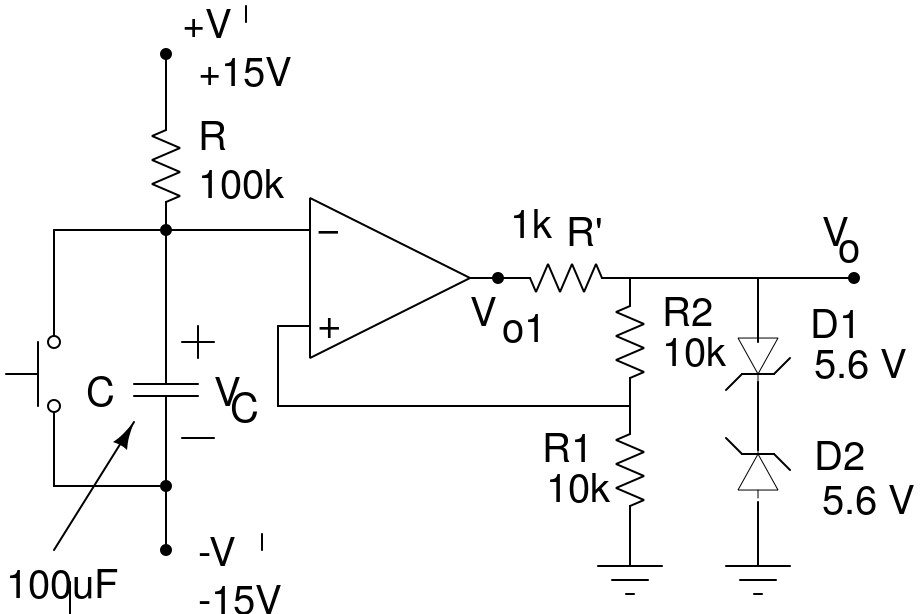
\includegraphics[width = 0.6\linewidth, height = 3in]{reports/lab2/mono.png}
            \caption{Monostable multivibrator}
        \end{figure}
       The actual resistance of resistors shown in fig 11 are,
        $R_1 = 9.7k$, $R_2 = 9.82k$, $R' = 0.99k$, $R = 100.5k$\\
        The voltage to which the capacitor charges is $2V' = 10.6V$\\
        \newpage
    The output pulse width, T is given by the expression
      \begin{align*} 
            T & = RC \times \log(\frac{V'}{V'-V_{TH}})\\
              & = (100.5k)\times(100\mu)\times\log(\frac{5.3}{5.3-3.4})
      \end{align*}
      \begin{equation}
            \boxed{T = 10.25s}
      \end{equation}
      
      \begin{figure}[H]
            \centering
            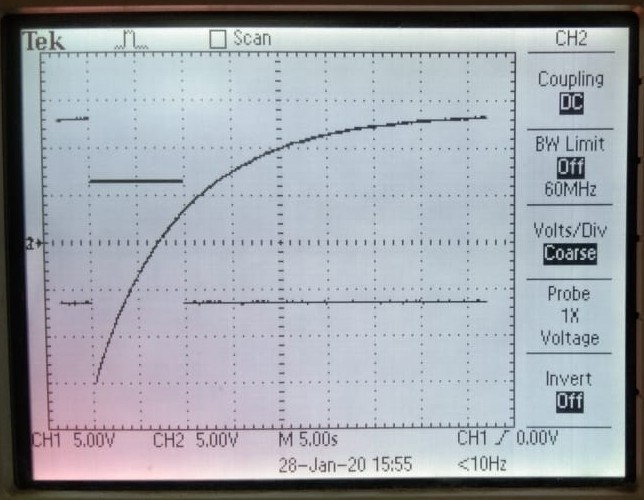
\includegraphics[width = 0.6\linewidth, height = 3in]{reports/lab2/monostable.jpeg}  
            \caption{Waveforms of $V_{-}$ and $V_{o}$}
        \end{figure}
      \\
    The observed pulse width comes out to be $\mathbf{T = 10.1s}$ 

\vspace{4cm}

    \begin{thebibliography}{9}

        \bibitem{Analog LAB Manual} 
        Scmitt supporting document 
        \\\texttt{https://moodle.iitb.ac.in/pluginfile.php/302403/mod\_resource/content/0/\\schmitt\_astable\_support.pdf}
        % \bibitem{Datasheet of UA741}
        % Datasheet of OpAmp UA741
        % \\\texttt{https://www.slideshare.net/YongHeuiCho/u-a741}
        
    \end{thebibliography}

\end{document}

